\documentclass{article}
\usepackage[fleqn]{amsmath}
\usepackage{amssymb,graphicx,color,graphicx,slashed, microtype, parskip, enumitem, extarrows, needspace}
%\usepackage[utf8x]{inputenc}
\usepackage[top=1.5cm, bottom=1.5cm, right=6cm, left=1.5cm, heightrounded, marginparwidth=5cm, marginparsep=0.5cm]{geometry}

\hbadness = 10000
\hfuzz=100pt 
    
\usepackage{marginnote}
\renewcommand*{\marginfont}{\footnotesize}

\usepackage{hyperref}
\hypersetup{colorlinks=true, urlcolor=NavyBlue, bookmarksdepth=3}

\makeatletter\newcommand{\@minipagerestore}{\setlength{\parskip}{\medskipamount}}\makeatother

% =============== Index ===========================

\usepackage[nonewpage]{imakeidx}
\makeindex

% =============== Color Definitions ===============
    
\usepackage[svgnames]{xcolor}
\colorlet{ColorTitle}{Black}
\colorlet{ColorSectionName}{Black}
\colorlet{ColorBoxFG}{Gray}
\colorlet{ColorBoxText}{Black}
\colorlet{ColorBoxBG}{White}


% =============== Title Style ===============
    
\usepackage{titling} % Allows custom title configuration
    
\newcommand{\HorRule}{\color{ColorTitle}\rule{\linewidth}{1pt}} % Defines the gold horizontal rule around the title
    
\pretitle{
    \vspace{-50pt} % Move the entire title section up
    \HorRule\vspace{9pt} % Horizontal rule before the title
    \fontsize{27}{36}\usefont{OT1}{phv}{b}{n}\selectfont
    \color{ColorTitle} % Text colour for the title and author(s)
}
    
\posttitle{\par\vskip 15pt} % Whitespace under the title
    
\preauthor{\fontsize{17}{0}\usefont{OT1}{phv}{m}{n}\selectfont\color{ColorTitle}} % Anything that will appear before \author is printed
    
\postauthor{\par\HorRule}

\newcommand{\COURSENAME}{\href{http://phyw.people.ust.hk/teaching/PHYS2022-2015/}{\textcolor{black}{PHYS 2022}}}
\newcommand{\YW}{\href{http://phyw.people.ust.hk/}{\textcolor{black}{Yi Wang}}}
\newcommand{\PHYS}{\href{http://physics.ust.hk}{\textcolor{black}{Department of Physics}}}
\newcommand{\HKUST}{\href{http://www.ust.hk/}{\textcolor{black}{HKUST}}}
\author{\COURSENAME, \YW, \PHYS, \HKUST}

\date{}

% =============== Section Name Style ===============
    
\usepackage{titlesec}
    
\titleformat{\section}
    {\fontsize{15}{20}\usefont{OT1}{phv}{b}{n}\color{ColorSectionName}}
    {\thesection}{1em}{}
    %[{\vspace{0.2cm}\titlerule[0.8pt]}]
    
\titleformat{\subsection}
    {\fontsize{14}{20}\usefont{OT1}{phv}{m}{n}\color{ColorSectionName}}
    {\thesubsection}{1em}{}
    
\titleformat{\subsubsection}
    {\fontsize{12}{20}\usefont{OT1}{phv}{m}{n}\color{ColorSectionName}}
    {}{0em}{}
      
\setcounter{secnumdepth}{4}
        
% =============== Box Style ===============
    
\usepackage[most]{tcolorbox}
    
\newtcolorbox{tbox}[1]{
    colback=ColorBoxBG, colframe=ColorBoxFG, coltext=ColorBoxText,
    sharp corners, enhanced, breakable, parbox=false,
    before skip=1em, after skip=1em,
    title={#1}, fonttitle=\usefont{OT1}{phv}{b}{n}, 
    attach boxed title to top left={yshift=-0.1mm}, boxed title style={sharp corners, colback=ColorBoxFG, left=0.405cm},
    rightrule=-1pt,toprule=-1pt, bottomrule=-1pt
}

\newtcolorbox{mtbox}[1]{
    colback=ColorBoxBG, colframe=ColorBoxFG, coltext=ColorBoxText,
    sharp corners, enhanced, breakable, parbox=false,
    before skip=1em, after skip=1em,
    title={#1}, fonttitle=\usefont{OT1}{phv}{b}{n},
    attach boxed title to top left={yshift=-0.1mm}, boxed title style={sharp corners, colback=ColorBoxFG, left=0.15cm},
    rightrule=-1pt,toprule=-1pt, bottomrule=-1pt, 
    left=0.5em
}

% =============== tikz has to be loaded after xcolor
\usepackage{tikz}

\newcommand*\enumlabel[1]{\tikz[baseline=(char.base)]{
			\node[shape=rectangle,inner sep=2pt,fill=ColorBoxFG] (char) 
			{\fontsize{7}{20}\usefont{OT1}{phv}{b}{n}{\textcolor{ColorBoxBG}{#1}}};}}

% =============== Useful shortcuts ===============

\newcommand\wref[1]{{\hypersetup{linkcolor=white}\ref{#1}}}  

\newcommand{\textbox}[2]{
    \begin{tbox}{#1}
        #2
    \end{tbox}
}

\newcommand{\mtextbox}[2]{\marginnote{
    \begin{mtbox}{#1}
        #2
    \end{mtbox}}
}

\newcommand{\mnewline}{\vspace{0.5em}\newline}

\newcommand{\titem}[1]{
    \begin{itemize}[label=\color{ColorBoxFG}$\blacktriangleright$, leftmargin=0mm, labelsep=0.27cm, topsep=0.5em
        %, itemsep=1ex
        ]
        #1
    \end{itemize}
}

\newcommand{\mtitem}[1]{
    \begin{itemize}[label={\color{ColorBoxFG}$\blacktriangleright$}, leftmargin=0mm, labelsep=1mm, topsep=0.5em
        %, itemsep=1ex
        ]
        #1
    \end{itemize}
}

\newcommand{\itembox}[3]{
    \begin{tbox}{#1}
        #2
        \titem{#3}
    \end{tbox}
}

\newcommand{\mitembox}[3]{
    \marginnote{
    \begin{mtbox}{#1}
        #2
        \mtitem{#3}
	\end{mtbox}
    }
}

\newcommand{\tenum}[1]{
    \begin{enumerate}[label=\protect\enumlabel{\arabic*}, leftmargin=0mm, labelsep=0.265cm, topsep=0.5em
        %, itemsep=1ex
        ]
        #1
    \end{enumerate}
}

\newcommand{\enumbox}[3]{
    \begin{tbox}{#1}
        #2
        \tenum{#3}
    \end{tbox}
}

\newcommand{\twocol}[5]{
    \begin{minipage}[t][][b]
        {#1\textwidth}
        #4        
    \end{minipage}
    \hspace{#2\textwidth}
    \begin{minipage}[t][][b]
        {#3\textwidth}
        #5
    \end{minipage}
}

\newcommand{\cg}[2]{
    \begin{center}
        \includegraphics[width=#1\textwidth]{#2}
    \end{center}
}

\newcommand{\tbar}{
    ~\newline
    {\color{ColorBoxFG}
    \hbox to 0.15\textwidth{\leaders\hbox to 5pt{\hss  \hss}\hfil} 
    \hbox to 0.7\textwidth{\leaders\hbox to 5pt{\hss . \hss}\hfil}}
    \mnewline
}

% =============== Filter unwanted warnings
\usepackage{silence}
\WarningsOff[tcolorbox]
\hbadness=1000000


\graphicspath{{2_fig/}}
\usepackage{wasysym}
\title{第二章\ 广义相对论}

\usepackage{ctex}

\begin{document}

\maketitle

\textbox{我们的地球拥有万有引力。所以——}{
    \tenum{
        \item 你楼上的邻居能比你更快收到订单。
        \label{item:high-fast}
        \item 站在你面前的人实际上比看起来矮。
        \label{item:person-short}
        \item 考虑一个三角形,它的边是最短距离线。如果水平握住它,其内角之和大于$180^\circ$;如果垂直握住它,则小于 $180^\circ$。
        \label{item:inner-angle}
    }
    \tcblower
    这些影响太小而无法注意到,因为地球引力很弱。如果地球质量特别大,不仅上述影响更加剧烈,而且
    \tenum{
        \setcounter{enumi}{3}
        \item 大地会变黑。此外,地球可以变得比现在更亮。
        \label{item:black-horizon}
        \item 如果你再靠近一点,地球的中心就不再是太空中的任何地方。它会成为你的未来。
        \label{item:singularity}
    }
}

所有这些都是由于重力。但是让我告诉你一个秘密——重力实际上不存在。

\section{等价原理}

\textbox{你和牛顿丢下一根羽毛和一块石头}{
    如果你在真空中丢下一根羽毛和一块石头,它们会以相同的加速度下落。你对这个事实感到惊讶吗?

    也许你小时候很惊讶,但在你学习了牛顿\footnote{Isaac Newton(1642-1726),英格兰物理学家、数学家、天文学家、自然哲学家和炼金术士。——译者注。}力学之后就不会再惊讶了。很显然:

    \twocol{0.4}{0}{0.3}{
        \titem{
            \item 牛顿第二运动定律: $F=ma$.
            \item 牛顿万有引力定律: $F=mg$.
        }    
    }{  
        $$ \Rightarrow \mbox{对于所有物质,} \quad a=g  $$
    }
    \tcblower
    但是牛顿并不觉得这很显然。 在 \textit{自然哲学的数学原理}中, 他写道:\marginnote{钟摆实验是一个测试物体如何坠落的更聪明的方法,因为它速度较慢且具有周期性。}
    \begin{quote}
         所有种类的重物体(除去空气的微小阻力造成的不等性和减速;质量由 $F/a$ 定义)从相同的高度落到地面的时间相等;而时间的相等性是由摆以很高精度测定的 $\ldots \ldots  \ldots $ 我曾用金、银、铅、玻璃、沙子、食盐、木块、水和小麦做过实验。
    \end{quote}
    为什么牛顿在这里非常小心?
}

\needspace{.2\textheight}
\mtextbox{重力很特别}{重力在这里很特别。力并不总是与质量成正比。电力 $F=qE$ 与物质的电荷成正比,而不是与质量成正比。所以对于电力来说,力的强度由电荷决定,惯性由质量决定。它们的比例因不同种类的物质而异。但是对于重力,它的强度和惯性都与质量成正比。}
\textbox{为什么重力的强度和惯性都能由质量决定?}{
要了解牛顿为何如此谨慎,就让我们来仔细地研究质量的含义吧。我们可以定义两个量:
    \titem{
        \item 惯性质量\index{惯性质量}: $m_I=F/a$ 是惯性的度量——改变速度的惰性。
        \item 重力质量\index{重力质量}: $m_G=F/g$ 重力——吸引物质的强度。
    }
    因此,$m_I$ 和$m_G$ 来自不同的来源。然而,牛顿断言 $m_I=m_G$。最先进的实验表明 $|(m_I / m_G)-1|<10^{-16}$。与其接受 $m_I=m_G$ 作为实验规则(实际上,实验规则有无数个——分别是金、银、铅、玻璃……),好奇的人想问:
    \titem{
        \item 等价性 $m_I=m_G$ 是否有普遍解释?
        \item 为什么重力如此特殊,而其他力则没有这样的等价性?
    }
}

爱因斯坦\footnote{Albert Einstein(1879-1955),犹太裔理论物理学家。——译者注。}回答了这些问题。猜猜他是怎么回答他们的? 1907年,爱因斯坦一生中``最幸福的思想''到来了——``如果一个人自由下落,他就不会感觉到自己的重量。''让我们来探索一下这个想法的力量。

\textbox{爱因斯坦的等效原理}{\index{等效原理}
    1907 年,爱因斯坦断言,对于均匀引力场:
    \mtextbox{对于非均匀重力}{如果引力场不均匀,只要观察者和所考虑的物理过程位于足够小的体积内,引力场就可以近似为均匀的。但是如果我们研究一个大系统,其中重力随位置的变化很重要,那么我们可能不仅依赖等效原理,还需要引入曲率的概念。
}

    ``我们$\ldots$ \textit{假定}(均匀)引力场和参考系的相应加速度的完全物理等效性。 ''

    例如,如果王二在电梯里,没有看外面。然后她发现以下情况没有变化:

    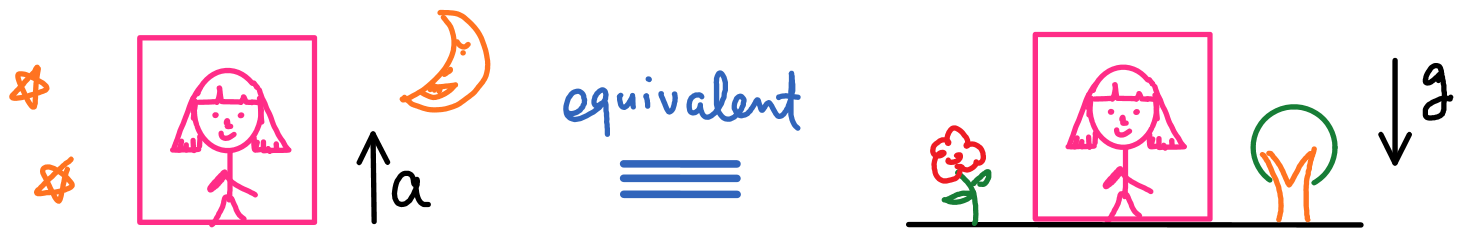
\includegraphics[width=1\textwidth]{ep}

    \tenum{
        \item 在没有重力的环境中电梯具有恒定加速度 $a$ 的升力
        \item 电梯没有移动,而是放置在引力场 $g=-a$ 中。
    }
    \tcblower
    我们在爱因斯坦的话中添加了``统一''以使其更加精确。如果引力场不均匀,我们总是可以研究空间中足够小的空间元素,其中引力场是均匀的。 (如何将这些小元素``拼凑''在一起很重要,因为这些元素可以导致时空弯曲。)
    \mtextbox{为什么作出这个假设}{每个人都可以做出假设。为什么这个是特别的?这个假设有着双重意义:
    \mtitem{
        \item 狭义相对论限制了我们对惯性系的关注。加速框架拓宽了相对论的范围。
        \item 重力从``常规''力降级为从根本上等同于虚构惯性力的东西。
    }}
}
这个假设确实回答了以下问题:$m_I=m_G$ 因为惯性(加速度)等于重力。引力是特殊的,因为这是这个基本假设中的力。


在这里,我们列举了一些假设的简单结果,并将更令人惊讶的结果留在后面的部分,因为它们需要更多的说明。

\textbox{匀加速可以抵消均匀重力}{
     这是因为均匀重力$g$等价于恒加速度$a=-g$,恒加速度$-g$可以被恒加速度$g$抵消。
    
    例如,人们在自由落体升降机或绕地球运行的卫星中感觉不到重力。这些观察者实际上可以将自己视为惯性系。对于这些观察者来说,均匀重力场可以被认为是不存在的(因为它不能被任何实验探测到)。

    因此(均匀)重力确实是特殊的(与所有其他力,如 E\&M 相比)——它和惯性力一样虚构。它的存在(或不存在)取决于观察者。
}
\mtextbox{星星、光线弯曲和透镜}{
    出于类似的原因,光在靠近物体(例如恒星或星系)时也会弯曲。由于恒星的引力场是不均匀的,因此不能仅根据等效原理来计算弯曲角。根据广义相对论的计算,弯曲角度是天真地应用等效原理的计算结果的两倍。这个弯曲角度是广义相对论的第一个验证预测(1915年)。
    \mnewline
    也可以另一种方式观察光线弯曲效果:物体像镜头一样聚焦光线。这种效应被称为 \textit{引力透镜}\index{引力透镜}。引力透镜被很好地观察到,并已成为了解我们宇宙物质分布的有力工具。
}
\textbox{光在均匀重力下弯曲\index{光的弯曲}}{
    光在均匀引力场中如何运动?这个问题在牛顿力学中可能被认为是没有明确定义的,因为光的质量为零(在相对论中,只有零质量的物体才能以有限的能量以光速运动)。但是根据等效原理,我们立即知道光的弯曲方式与加速环境中的弯曲方式相同。这解释了本部分开头给出的事例\ref{item:person-short} 。
}

\section{均匀重力时间}

回想一下,在孪生悖论中,加速会产生王二和王三之间的物理时间差(因为王二必须加速返回才能再次见到王三)。现在加速度等于均匀重力,我们预计重力也会在观察者之间造成一些时间差异。我们将看到情况确实如此。

\textbox{更高即更远}{
    现在王二比王三高一个垂直距离$h$。重力加速度为 $g$。王二的时间流逝和王三的时间流逝有什么不同吗?
    
    为了量化``时间流逝'',考虑王二发送两个间隔为 $\Delta t_A$ 的光脉冲。王三收到这两个脉冲的时间间隔是多少?

    为了更简便地计算,我们假设 $c\Delta t_A \ll h$ 和 $gh\ll c^2$。这种情况如下图的左侧面板所示。

    \cg{0.6}{ep_time}

    \tcblower
    
    为了解决这个问题,我们利用了等价原理。该系统相当于下图右侧面板中的情况:没有重力。而是王二和王三以加速度 $a=g$ 向上加速。
    
    我们设$t=0$为王二发出第一个信号的时间,也是王二和王三速度$v=0$的时间。让光信号的空间分离为$s$。请注意,$s$ 应该是一个常数,因为没有重力或其他影响光传播的力。

    关于王二,当她发送信号时,她的速度是 $v=0$,因此 $s= c\Delta t_A$。

    \marginnote{我们在王三的位置请了第三位观察者C静止研究王三关于光信号的运动。如果要说王三的时间间隔是什么,其实她和观察者C之间是有时间膨胀效应的。但是时间膨胀效应是$v^2/c^2$级的,所以在这个分析中很小。}
    关于观察者关于王三的位置是静置的,当王三接收到信号时,他的速度为 $v = a h/c$。请注意,光信号和王三正在朝着对方移动。因此$s = (c+v)\Delta t_B$。因此
    \begin{align}
        \Delta t_A = \left ( 1 + \frac{ah}{c^2}  \right ) \Delta t_B~.
    \end{align}
    因此,王三发现王二更快。王二越高越快。如果在$t=0$ 王二 和王三的年龄相同,之后王二会发现王三更年轻,王三会发现王二更老。

    这解释了本部分开头给出的事例 \ref{item:high-fast}。
}

\mtextbox{再次出现孪生悖论}{现在我们可以使用旅行双胞胎的框架来解释双胞胎悖论。旅行中的双胞胎需要在返回前加速。如果我们将加速度建模为匀加速,那么由于等效原理,对应于引力势。然后静态双胞胎在这种引力势中就突然变老了。}
\textbox{具有引力势的时间膨胀}{\index{引力时间膨胀}
    更一般地说,对于处于引力势 $\phi$ 中的王二和王三,时间膨胀可以用它们的引力势差表示为
    \begin{align}\label{eq:gr-phi}
        dt_A = \left ( 1 + \frac{\phi_A - \phi_B}{c^2}  \right ) dt_B ~.
    \end{align}
}


\textbox{球形恒星的度量}{\index{引力时间膨胀}
    考虑质量为 $M$ 的球形恒星。令王三在 $r\rightarrow \infty$,即令她远离恒星。那么王三不会受到来自恒星的引力,并且有$\phi_B=0$。因此我们可以将王三的时间视为没有恒星引力的标准时间:$t_B = t$。
    
    而王二具有引力势$\phi_A=-GM/r$。使用方程~\eqref{eq:gr-phi},我们得到\marginnote{注意,恒星的引力场是不均匀的。不过好在 Eq.~\eqref{eq:gr-phi} 在这里还是可以用的。这甚至在重力非常强的情况下也成立。这个说明(解出恒星的爱因斯坦方程)超出了这个简短介绍的范围。}
    \begin{align}
        dt_A = \left ( 1 + \frac{\phi_A}{c^2}  \right ) dt~.
    \end{align}
    对于王二静止在恒星的固定位置,$d\mathbf{x}=0$,并且
    \begin{align}
        \label{eq:ds2-schwarzschild}
        ds^2 = - c^2 (\mbox{proper time})^2  = - c^2 dt_A^2 
        = - \left ( 1 + \frac{2\phi_A}{c^2}  \right ) c^2 dt^2~. 
      \end{align}
      \mtextbox{加速度和空间曲率}{
          爱因斯坦指出,为了协调加速坐标系和狭义相对论,必须引入弯曲 3d 空间的概念。例如,王二在做匀速圆周运动,王三站在圆心。王二和王三在圆的半径上一致,但在圆周上不一致。因此,王二的空间应该是弯曲的。
          \tcblower
          在弯曲的空间中,比如在一个球体内,你可以画一个三角形并测量内角的总和。你得到了什么?这解释了本部分开头给出的事例\ref{item:inner-angle} 。
      }
      一般来说,$d \mathbf{x}^2$前面的系数(即度量的空间部分)也会被修改。我们这里只给出结果:\index{史瓦西度规}
      \begin{align}
        \label{eq:schwarzschild}
        ds^2 = - \left ( 1 - \frac{r_s}{r}  \right ) c^2 dt^2
        + \left ( 1 - \frac{r_s}{r}  \right )^{-1} dr^2
        + r^2 \left ( d\theta^2 + \sin^2\theta d\phi^2 \right )~,
      \end{align}
      这被称为史瓦西度规,描述了球对称恒星外部的时空几何。它的半径
      \begin{align}
        \label{eq:rs}
        r_s \equiv \frac{2GM}{c^2} 
      \end{align}
      被称为史瓦西半径。
}

\textbox{Example: The sun}{
    为公式~\eqref{eq:rs} 代入数字,如果$M$ 是太阳质量,则$r_s = 3$km。这 3 公里的距离对太阳意味着什么?

    \tcblower

    这并不意味着什么。因为太阳半径是$r_\odot = 7\times 10^5$km。史瓦西度规\eqref{eq:schwarzschild}仅适用于恒星外部,因为在恒星内部,引力势的形式采用不同的形式。

    然而,如果一个物体如此密集,以至于它的半径小于$r_s$呢?例如,如果一个物体的质量与太阳相同,但半径小于 3 公里怎么办?

}

\section{黑洞}

现在想象一个物体非常密集,以至于它的大小小于其史瓦西半径 $r_s = 2GM/c^2$。然后会发生什么?

事实上,这不是一个只存在在想象中的问题。如此密集的物体——黑洞——是真实存在的。从天体运动的分析到对它的形状进行成像,再到引力波的观测,许多观测方法都可以检测到它们。

\textbox{$r=r_s$ 附近会发生什么?}{
    When $r\simeq r_s$, in Eq.~\eqref{eq:schwarzschild} the time part vanishes and the spatial part blows up. What's happening there?当 $r\simeq r_s$ 时,在 Eq.~\eqref{eq:schwarzschild} 中,时间部分消失,空间部分爆炸。那里发生了什么事?

    想象
    \mtextbox{二元性和全息}{王二 sees herself falling across $r_s$ but 王三 sees 王二 frozen at $r_s$. We will explain that they do not have a chance to meet (up to quantum subtleties which remain open questions in research) and thus nothing goes wrong.类似于孪生悖论,现在王二和王三有一个分歧:王二看到自己跌倒在 $r_s$ 上,但王二看到王二被冻结在 $r_s$ 处。我们将解释他们没有机会见面(直到在研究中仍然悬而未决的量子微妙之处)这一说法将没有任何问题。
    \mnewline
    王三 sees and describes 王二 on the 2-dimensional surface $r=r_s$, while 王二 sees and describes herself in a 3-dimensional volume $r<r_s$. The two descriptions \textit{may} be equivalent to each other. This conjecture is known as holography in theoretical physics as the dual descriptions are between a surface and a volume.王三在二维表面 $r=r_s$ 上看到并描述了王二,而王二在三维体积 $r<r_s$ 上看到并描述了自己。这两个描述 \textit{可能} 彼此等效。这个猜想在理论物理学中被称为全息,因为双重描述存在于表面和体积之间。
    }
    王二保持的距离$r$只比$r_s$大一点点。重力试图把她拉下去,但想象她在拥有强大推力的火箭中,以保持她保持在固定的 $r$。而王三位于 $r\rightarrow \infty$。对于根据王二的任何有限区间 $\Delta t_A$,对于王三:
    \begin{align}
        \Delta t_B = \Delta t_A \times \left ( 1 - \frac{r_s}{r}  \right )^{- \frac{1}{2} } \rightarrow \infty~.
    \end{align}
    因此,王三发现王二冻结在 $r=r_s$ 表面上。一般而言,在 $r \rightarrow r_s$ 处,引力膨胀效应非常显着,以至于对于外部观察者来说,时间看起来都冻结了。关于这个效应,如果你旅行接近 $r\rightarrow r_s$ ,然后返回,引力膨胀效应会成为一个带你去往未来的时间机器。
    \tcblower
    以上是王三的发现。但是对于王二,她并不觉得$r=r_s$很特别。在任何时刻,假设她比 $r_s$ 小得多,等价原理告诉她,她的加速度抵消了她的重力,她只是在有限的时间内从外到内穿过 $r=r_s$。
}

\textbox{``事件视界''和``黑洞''}{
    对于 $r<r_s$ 的事件,王三会看到什么?例如,王二穿过$r_s$到达$r<r_s$后,王二能看到什么?

    看不到任何东西。
    \mtextbox{黑洞真的是黑色的吗?}{
        并不是。
        \tcblower
        \mtitem{
            \item 理论上,来自量子引力的霍金辐射可以来自黑洞。它们通常太暗而看不见。
            \item Due to the emission of infalling matter, images of black holes have been taken by arrays of radio telescopes in 2019.实际上,有些黑洞是我们宇宙中最亮的天体——可没有开玩笑。落入黑洞的物质(无限深的引力势)相互作用并发出明亮的辐射——高达$40\%$的物质能量可以转化为光。由于下陷物质的发射,2019年的射电望远镜阵列拍摄了黑洞的图像。
        }
    }
    由于极端的时间膨胀,在 $r_s$ 发出的光需要无限的时间才能到达王三。王三不能拥有无限的等待时间,因此在 $r<r_s$ 处看不到任何事情。

    因此,$r=r_s$ 是限制王三可以看到的事件的表面。故$r=r_s$ 被称为\textit{事件视界}\index{事件视界}。密集的物体隐藏在这个事件视界内,因此是不可见的。来自该物体的光无法到达外部。因此,该物体被称为 \textit{黑洞}\index{黑洞}。这解释了本部分开头给出的事例 \ref{item:black-horizo​​n}。
}
 
\textbox{在视界``内部'':未来将在奇点处消失}{
    王二掉进黑洞(穿过$r=r_s$视界)后会发生什么?

    Wrt 王三, he cannot expect to see 王二 coming out again. Since when she crosses the horizon, it already corresponds to $t_B\rightarrow \infty$. 王三 can see nothing happening later than infinity.对于王三来说,王二不能再次出现。因为当她穿过地平线时,它已经对应于 $t_B\rightarrow \infty$。王三在无穷之后什么也看不到。

    但是对于王二自己,她为什么不能决定用她的火箭来逃离视界呢?
    \tcblower
    为了回答这个问题,让我们来看看史瓦西度量
    \eqref{eq:schwarzschild}. At $r<r_s$, the metric can be rewritten as
    \begin{align}
        \label{eq:schwarzschildIn}
        ds^2 = 
        - \left ( \frac{r_s}{r} -1 \right )^{-1} dr^2
        + \left (  \frac{r_s}{r} -1  \right ) c^2 dt^2
        + r^2 \left ( d\theta^2 + \sin^2\theta d\phi^2 \right )~.
    \end{align}
    \marginnote{这解释了本部分开头给出的事例 \ref{item:singularity}。}
    What happened? Now $dr$ is time-like and $dt$ is space-like! The time direction and one space direction have flipped their roles. For 王二, the $-r$ direction is now the time direction.现在发生了什么?现在 $dr$ 是类似时间的,而 $dt$ 是类似空间的!时间方向和空间方向发生了翻转。对于王二来说,$-r$ 方向现在是时间方向。

    The time direction is special since it is one-way. You can choose to move left or right in space, but have no choice but moving forward in time. Now 王二 has no choice other than to move along her time direction (the direction to reduce $r$) towards $r=0$, regardless the spatial direction (now $t, \theta, \phi$) that 王二 would like to travel.时间方向是特殊的,因为它是单向的。你可以选择在空间上向左或向右移动,但在时间上别无选择。现在王二别无选择,只能沿着她的时间方向(减少 $r$ 的方向)朝向 $r=0$喜欢旅游。

    不仅王二,黑洞内的一切,包括致密物体本身,都在$r=0$处落向未来。他们的时间在这里便结束了,因此它被称为 \textit{singularity}\index{singularity}。事实上,按照广义相对论的计算,在到达奇点之前,每个物体都会由于奇点附近的发散潮汐力而被撕裂。

    在黑洞内部,奇点一定会和经典广义相对论扯上关系。如何用完整的理论中理解和表示这种奇点仍然是一个悬而未决的问题,而且该理论应该可以以一致的方式(量子引力)描述引力和量子力学。
}

\section{引力波}\index{gravitational waves}

引力波是广义相对论完整理论的产物。如果要严格地推导它们会超出我们将要讲的范围。尽管如此,我们会在这里建立一些直观的理解。

\textbox{狭义相对论和牛顿引力不一致}{
    传统的牛顿引力 $F = G_N Mm / r^2$ 有什么问题?

    假设王二距离王三一光年,她挥手。随着她手的位置 $r$ 的变化,原则上王三可以测量出与王二\emph {immediately}略有不同的引力——因为力不需要时间在牛顿引力中传播。王二因此可以将信息编码在她的手如何移动中,并立即将信息发送给王三。这比光还快。

    从狭义相对论来看,没有任何信息可以比光速传播得更快。因此,牛顿引力不符合狭义相对论。

    从概念上讲,用时空曲率代替重力并不能解决这个问题。举个例子,当你移动你的手时,时空曲率是否能以比光还快的速度变化?
}

\mtextbox{引力波的早期历史}{
    回到 1893 年,Oliver Heaviside 回到 1893 年,黑维塞\footnote{Oliver Heaviside(1850-1925),英国物理学家和电子工程师。——译者注。}注意到引力和 E\&M 的相似性,并提出引力可能以波的形式传播。但只有在广义相对论建立后,引力波的讨论才被纳入合适的科学框架。爱因斯坦于1916年第一个根据他的广义相对论预测了引力波。
}
\textbox{What gravity can learn from E\&M?从 E\&M 中可以学习到什么引力?}{
    In Newtonian gravity, you can send superluminal information by waving your hands and detect the force change using $F=G_N Mm /r^2$. However, why don't E\&M have the same problem with Coulomb force $F\propto Qq/r^2$?在牛顿引力中,你可以通过挥手发送超光速信息,并使用 $F=G_N Mm /r^2$ 检测力的变化。但是,为什么E\&M没有库仑力$F\propto Qq/r^2$同样的问题呢?
    \tcblower
    If we only have the Coulomb force formula and nothing else, we would have the same superluminal problem for E\&M. However, the magnetic field comes to rescue here. Once the source electric charge accelerates (you cannot encode information by inertial motion without acceleration), the time variation of the electric field produces magnetic field, and the time variation of the magnetic field produces electric field. This process happens over and over again and E\&M wave is emitted at exactly the speed of light. Also, in this way, the E\&M field can propagate by itself without the need of matter (after produced by a source) as new ``degrees of freedom''.如果我们在这里只有库仑力方程,那么 E\&M 就会遇到同样的超光速问题。然而,磁场在这里起到了拯救作用。一旦源电荷加速(没有加速就不能通过惯性运动编码信息),电场的时间变化产生磁场,磁场的时间变化产生电场。这个过程一遍又一遍地发生,E\&M 波以完全光速发射。此外,通过这种方式,E\&M 场可以在不需要物质(由源产生之后)作为新的“自由度”自行传播。

    The lesson: we hope that new ``degrees of freedom'' can come to rescue in gravity, similar to what magnetic field does for E\&M. Where to find those degrees of freedom?思考:我们希望新的“自由度”可以在重力中解救,类似于磁场对 E\&M 的作用。在哪里可以找到这些自由度?
    % 内部注释:细节:重力电磁学。见例如:
    % https://arxiv.org/pdf/gr-qc/0003115.pdf
    % https://arxiv.org/pdf/gr-qc/9912027.pdf
}

\needspace{.22\textheight}
\mtextbox{引力波是具有物质属性的吗?}{
     令人担忧的是,空间会变形,尺度也会变形。那么我们真的可以测量引力波吗?这场争论持续了 40 年。 1957 年,费南(化名``史密斯先生'')认为,当引力波通过时,棒上的水滴会相对于棒移动,从而通过摩擦产生热量。因此引力波具有物质属性的。观测工作随即开始。 2016 年,经历了数十年的追踪和失败,引力波终于被激光干涉引力波天文台 (LIGO) 使用类似于迈克尔逊莫雷实验的干涉仪探测到了。
}
\textbox{选读:动力学度量和引力波}{
    We have shown that a static gravitational field can be described by a non-trivial metric, for example \eqref{eq:schwarzschild}. There are other components in the metric as well. The metric can be viewed as a $4\times 4$ symmetric matrix with 10 components (free functions to choose). 8 of them are already used:我们已经证明静态引力场可以用一个非显然的度量来描述,例如 \eqref{eq:schwarzschild}。度量中还有其他部分。该度量可以被视为具有 10 个分量(可供选择的自由函数)的 $4\times 4$ 对称矩阵。其中 8 个已经使用:
    \titem{
        \item 4 to describe the response to energy and momentum of matter. The energy part is the Newtonian gravity and the momentum part is its relativistic generalization. Technically they are called the Hamiltonian (energy) and momentum constraints.其中4个对称矩阵描述对物质能量和动量的反应。能量部分是牛顿引力,动量部分是它的相对论概括。用专业名词来说,它们被称为哈密顿量(能量)和动量约束。
        \item 4 represents the freedom to choose coordinates. When choosing any new coordinate system $\tilde x^\mu (x)$, we expect that the physical interval should not change and thus the metric should transform accordingly.另外4个对称矩阵代表自由选择坐标。在选择任何新坐标系$\tilde x ^\mu(x$时,我们希望物理间隔不应改变,因此度量标准应相应地转换。
    }
    剩下的 2 个自由度是什么?令人高兴的是,它们对应于传播的引力波,以解决牛顿引力问题。并且引力波以光速传播。
}

\marginnote{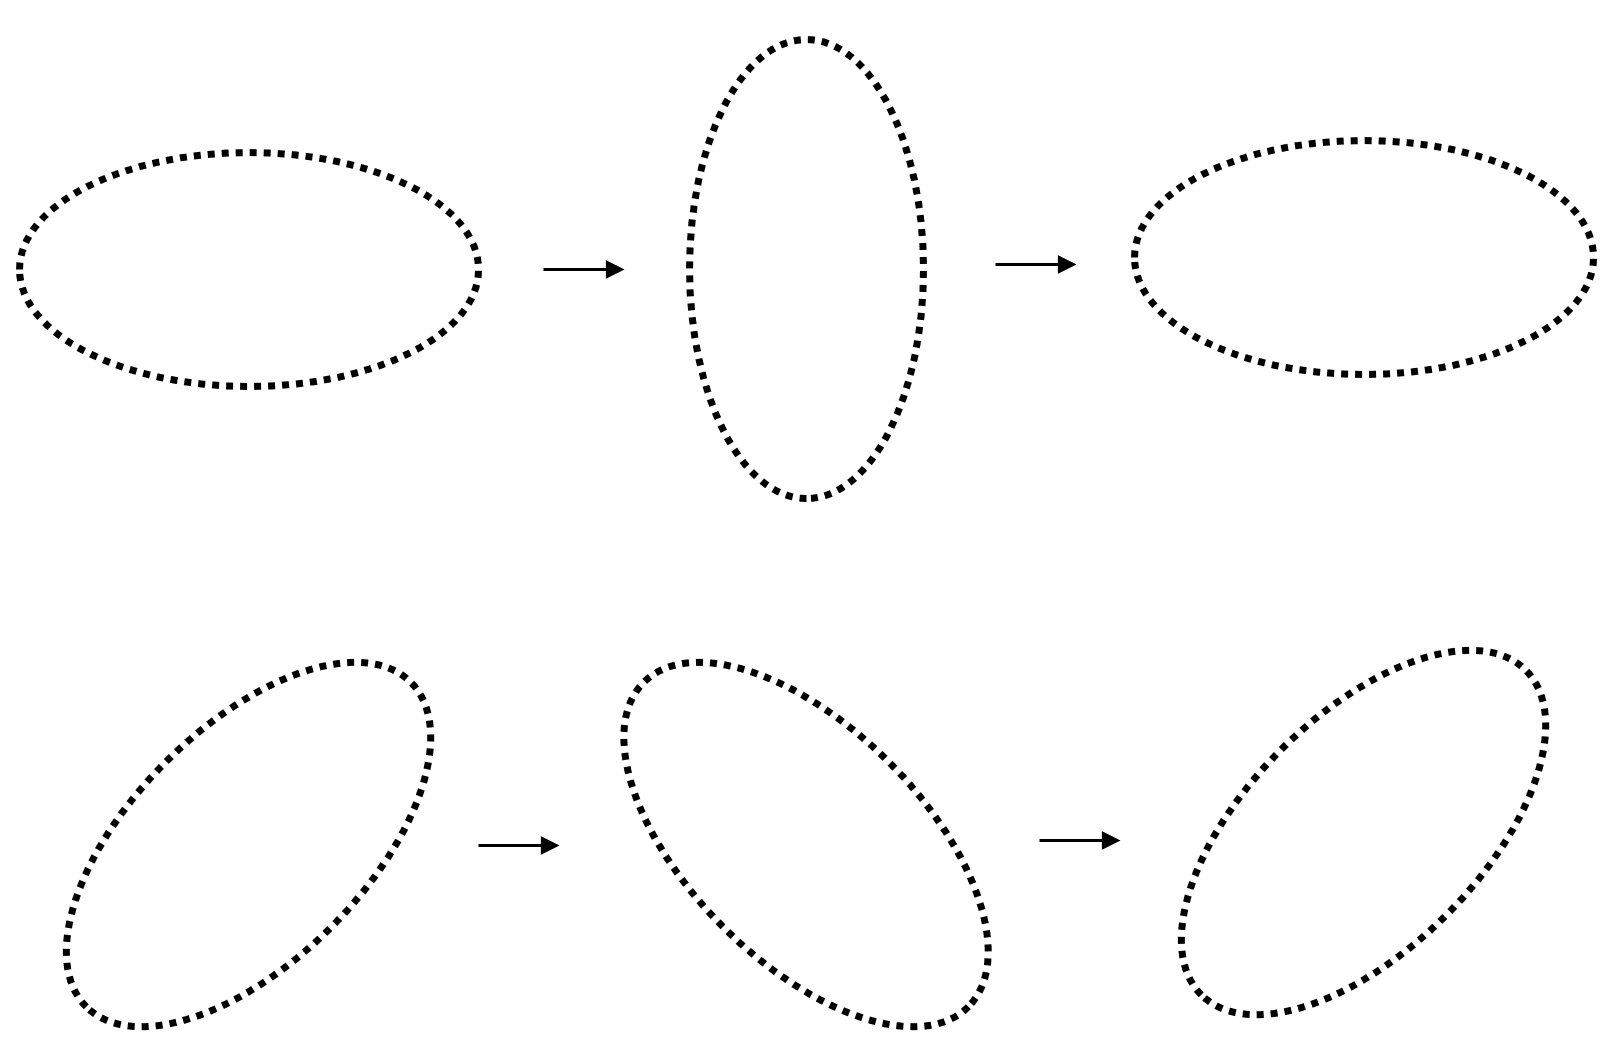
\includegraphics[width=0.35\textwidth]{gwpol}}
\textbox{引力波是什么样子的?}{
     正如我们已经讨论的,引力波是时空的波动,以度量为特征。因此,它们的影响应该是距离的扭曲。它们以光速传播,并且它们是横波(偏振垂直于传播方向)。两个独立的偏振模式使时空变形,如右图所示。
}

\section{结语:总结和下一步}

\textbox{科学中罕见的例子}{
    广义相对论是现代科学史上一个非常罕见的例子,它是一个全新的科学框架。它(几乎)完全是由逻辑推理和哲学信仰建立的。

    从等效原理开始,我们向你展示了时间如何在均匀引力场中变得相对。然后我们说明球形恒星也有类似的效果。如果恒星足够密集,就会形成黑洞。黑洞有一个事件视界,物质(经典,不考虑量子力学情况)可以进入但不能返回。从引力和 E\&M 之间的相似性来看,我们认为引力波是作为时空变形而存在的。所有这些都可以用微分几何的数学框架精确而优雅地表达出来。
}

等效原理是广义相对论中的第一个观察结果,但这还不是最精彩的。虽然超出了课程的范围,但让我们提一下广义相对论中的两个关键概念:

\textbox{空间是如何弯曲的?}{
    如何确定诸如 \eqref{eq:schwarzschild} 之类的几何?在牛顿引力中,我们知道引力是由物质分布决定的。既然引力被解释为几何学,几何学也应该由物质分布决定,至少在牛顿极限内。从物质分布确定几何的规则是爱因斯坦方程。它看起来像 $G_{\mu\nu} = 8\pi G T_{\mu\nu}$ \index{爱因斯坦方程},是广义相对论的主要方程。我们无法在本课程的范围内向你解释它,不过会提到方程左侧由度量 $g_{\mu\nu}$ 及其衍生物决定;而方程右侧是由物质分布决定的。这被称为``物质告诉空间如何弯曲''。
}

\textbox{物质是如何运动的?}{
    How matter moves in curved space? Matter follows the geometry of spacetime. This is dubbed ``space tells matter how to move.'' Given a spacetime geometry, the motion of free-falling matter is determined by a generalized version of the twin paradox. Recall that in the twin paradox, the free observer without external force exerted has the longest proper time. We assert that, free-fall observers in general relativity still have extrema (usually longest but there are exceptions that the proper time is only longest for a selection of variations) proper times. Such extremal paths are known as geodesics. A geodesic can be interpreted in a semi-Newtonian manner as follows: the equation of a geodesic is物质如何在弯曲空间中运动?物质遵循时空几何学运动,或者可以被称为``宇宙告诉物质如何运动''。给定一个时间-空间几何,自由落体物质的运动是由孪生悖论的广义版本决定的。回想一下,在孪生悖论中,没有施加外力的自由观察者的固有时间最长。我们断言,广义相对论中的自由落体观察者仍然具有极值(通常最长,但也有例外,正确时间仅对于选择的变体才是最长的)正确时间。这种极值路径称为测地线。测地线可以用半牛顿的方式解释如下:测地线的方程是 \index{geodesic equation} 这里 $a_\mu$ 是 4-加速度,$u^\alpha$ 是 4-速度。 $\Gamma^\mu_{\alpha\beta}$ 是引力概念的推广,由度量及其导数构成。你可能已经意识到这像牛顿第二定律。是否将方程右侧解释为重力,或几何学中的术语来说明物质如何运动,这完全取决于你。正如等价原则所表示的,它们是等价的。
}

\textbox{广义相对论是普遍适用的吗?}{
    以上两个原理是广义相对论的关键,广义相对论适用于所有已知的可以研究重力的尺度,包括实验室非常精确的重力实验的毫米尺度,到整个宇宙的大小。

    尽管如此,到目前为止,我们仍然不明白如何在量子力学的框架内建立广义相对论。寻找这样一个统一理论的努力被称为``量子引力''\index{量子引力}。实验还不够精确,无法探测引力的量子效应。但是广义相对论和量子力学之间的理论一致性也是一个动机很好而且出奇的难的问题。当前量子引力的主要候选者是弦论\index{弦论},它首先假设基本粒子实际上是一维空间而不是零维的弦(零对应于点粒子)。
} 

\textbox{扩展阅读}{
    有很多关于广义相对论的好书可以读。一些适合初学者的易读书籍有由哈妥\footnote{James B. Hartle(1939-),美国物理学家。——译者注。} 编写的 \href{https://www.amazon.com/dp/0805386629/?tag=stackoverfl08-20}{Gravity: An Introduction to Einstein’s General Relativity} 和舒茨\footnote{Bernard F. Schutz(1946-),美国物理学家。——译者注。}编写的 \href{https://www.amazon.com/First-Course-General-Relativity/dp/0521887054}{A First Course in General Relativity}
}


\section{练习}

1. 计算你在楼上变老的速度有多快。考虑狭义相对论和广义相对论的影响。

2. 考虑到现代卫星导航系统(如北斗、伽利略、GLONASS 或 GPS)的精度,如果不考虑这些因素,狭义相对论和广义相对论效应对这些卫星导航系统的精度有多大影响?

\printindex

\end{document} 